\documentclass{article}

\usepackage[T1]{fontenc}

\usepackage{fancyhdr}
\usepackage{extramarks}
\usepackage{amsmath}
\usepackage{amsthm}
\usepackage{amsfonts}
\usepackage{tikz}
\usepackage{algorithm}
\usepackage{algpseudocode}
\usepackage{enumitem}

\usepackage[mono=false]{libertine}


\usetikzlibrary{automata,positioning}

%
% Basic Document Settings
%

\topmargin=-0.45in
\evensidemargin=0in
\oddsidemargin=0in
\textwidth=6.5in
\textheight=9.0in
\headsep=0.25in

\linespread{1.1}

\pagestyle{fancy}
\lhead{\hmwkAuthorName}
\chead{\hmwkClass: \hmwkTitle}
\rhead{\firstxmark}
\lfoot{\lastxmark}
\cfoot{\thepage}

\renewcommand\headrulewidth{0.4pt}
\renewcommand\footrulewidth{0.4pt}

\setlength\parindent{0pt}

%
% Create Problem Sections
%

\newcommand{\enterProblemHeader}[1]{
    \nobreak\extramarks{}{Problem \arabic{#1} continued on next page\ldots}\nobreak{}
    \nobreak\extramarks{Problem \arabic{#1} (continued)}{Problem \arabic{#1} continued on next page\ldots}\nobreak{}
}

\newcommand{\exitProblemHeader}[1]{
    \nobreak\extramarks{Problem \arabic{#1} (continued)}{Problem \arabic{#1} continued on next page\ldots}\nobreak{}
    \stepcounter{#1}
    \nobreak\extramarks{Problem \arabic{#1}}{}\nobreak{}
}

\setcounter{secnumdepth}{0}
\newcounter{partCounter}
\newcounter{homeworkProblemCounter}
\setcounter{homeworkProblemCounter}{1}
\nobreak\extramarks{Problem \arabic{homeworkProblemCounter}}{}\nobreak{}

%
% Homework Problem Environment
%
% This environment takes an optional argument. When given, it will adjust the
% problem counter. This is useful for when the problems given for your
% assignment aren't sequential. See the last 3 problems of this template for an
% example.
%
\newenvironment{homeworkProblem}[1][-1]{
    \ifnum#1>0
        \setcounter{homeworkProblemCounter}{#1}
    \fi
    \section{Problem \arabic{homeworkProblemCounter}}
    \setcounter{partCounter}{1}
    \enterProblemHeader{homeworkProblemCounter}
}{
    \exitProblemHeader{homeworkProblemCounter}
}

%
% Homework Details
%   - Title
%   - Due date
%   - Class
%   - Section/Time
%   - Instructor
%   - Author
%

\newcommand{\hmwkTitle}{Homework\ \#6}
\newcommand{\hmwkDueDate}{April 24, 2018}
\newcommand{\hmwkClass}{Design and Analysis of Algorithms}
\newcommand{\hmwkClassInstructor}{Professor Kasturi Varadarajan}
\newcommand{\hmwkAuthorName}{\textbf{Alic Szecsei}}

%
% Title Page
%

\title{
    \vspace{2in}
    \textmd{\textbf{\hmwkClass:\ \hmwkTitle}}\\
    \normalsize\vspace{0.1in}\small{Due\ in\ class\ on\ \hmwkDueDate}\\
    \vspace{0.1in}\large{\textit{\hmwkClassInstructor}}
    \vspace{3in}
}

\author{\hmwkAuthorName}
\date{}

\renewcommand{\part}[1]{\textbf{\large Part \Alph{partCounter}}\stepcounter{partCounter}\\}

%
% Various Helper Commands
%

% Useful for algorithms
\newcommand{\alg}[1]{\textsc{\bfseries \footnotesize #1}}

% For derivatives
\newcommand{\deriv}[1]{\frac{\mathrm{d}}{\mathrm{d}x} (#1)}

% For partial derivatives
\newcommand{\pderiv}[2]{\frac{\partial}{\partial #1} (#2)}

% Integral dx
\newcommand{\dx}{\mathrm{d}x}

% Alias for the Solution section header
\newcommand{\solution}{\textbf{\large Solution}}

% Probability commands: Expectation, Variance, Covariance, Bias
\newcommand{\E}{\mathrm{E}}
\newcommand{\Cov}{\mathrm{Cov}}
\newcommand{\Bias}{\mathrm{Bias}}

% Set from 1 to N
\newcommand{\XYZ}[1]{\left\{1,\ldots,{#1}\right\}}
\newcommand{\Break}{\textbf{break} }
\newcommand{\Var}[1]{\textsf{#1}}

\begin{document}

\maketitle

\pagebreak

\begin{homeworkProblem}

For any flow network $G$ and any vertices $u$ and $v$ let $bottleneck_G(u,v)$ denote the maximum, over all paths $\pi$ in $G$ from $u$ to $v$, of the minimum-capacity edge along $\pi$.

\begin{enumerate}[label=(\alph*)]
\item Describe and analyze an algorithm to compute $bottleneck_G(s,t)$ in $O(E \log V)$ time. 
\end{enumerate}

\solution\\

\part 

\begin{algorithm}
	\begin{algorithmic}[1]
		\Function{Bottleneck}{$G, u, v$}
			\State $queue \gets$ an empty heap
			\State $current \gets u$
			\ForAll{$vertex$ in $G.vertices$}
				\If{$vertex = u$}
					\State $vertex.weight \gets \infty$
				\Else
					\State $vertex.weight \gets -\infty$
				\EndIf \Comment{We'll use these weights in our heap}
				\State insert $vertex$ into $queue$
			\EndFor
			\While{$\neg v.seen$} \Comment{Find the path with the bottleneck by building a tree}
				\State $current.seen \gets \Var{True}$
				\ForAll{$d$ in $current.neighbors$}
					\If{$\neg d.seen$}
						\If{$edge(current,d).weight > d.weight$}
							\State delete $d$ from $queue$
							\State $d.weight \gets edge(current, d).weight$
							\State $d.parent \gets current$
							\State insert $d$ into $queue$
						\EndIf
					\EndIf \Comment{Update the vertex weight of a neighbor of $current$}
				\EndFor
				\State $current \gets$ dequeue the max vertex in $queue$
			\EndWhile
			\State $c \gets v$
			\State $min \gets \infty$
			\While{$c \neq u$} \Comment{Find the minimal edge in the bottlenecking path}
				\If{$edge_{c, c.parent}.weight < min$}
					\State $min \gets edge_{c, c.parent}.weight$
				\EndIf
				\State $c \gets c.parent$
			\EndWhile
			\State \Return $min$
		\EndFunction
	\end{algorithmic}
\end{algorithm}

This assumes the function should return the \emph{weight} of the bottlenecking edge; however, it can trivially be modified to return the edge itself.\\

This algorithm is essentially a modification of Prim's algorithm, where instead of searching for minimally-weighted edges, we instead search for maximally-weighted edges. To do this, we use a priority queue (using a binary heap).\\

We can split up our algorithm into three sections. The first is where we add each vertex into the priority queue. This is a total of $V$ insertions into the queue, each of which takes $O(\log V)$ time, for a total runtime of $O(V \log V)$.\\

Second, we build a spanning tree in $G$ until we have found a route from $u$ to $v$. To do this, we continually dequeue vertices from our queue. For each unvisited neighboring vertex, we check if we've found a better edge to connect it to our tree. If so, we update the weight of the vertex, and also update its ``parent'' in the tree. We continue in this fashion until $v$ has been added to the tree. Each time we attempt to update a vertex, it means we have traversed a new edge in the graph; updating the vertex involves a successive deletion and insertion, both of which are $O(\log V)$. Since this can happen at most $E$ times, the total running time for this section is $O(E \log V)$.\\

Last, we determine the smallest edge in the path from $v$ to $u$. This is more straightforward, as it is a simple $O(E)$ loop.\\

Our total running time is thus $O((E + V)\log V)$; since $V$ is $O(E)$ for any connected graph, we can say that it is $O(E \log V)$.

\end{homeworkProblem}

\pagebreak

\begin{homeworkProblem}

Suppose you have already computed a maximum flow $f*$ in a flow network $G$ with \emph{integer} edge capacities.

\begin{enumerate}[label=(\alph*)]
\item Describe and analyze an algorithm to update the maximum flow after the capacity of a single edge is increased by 1.
\item Describe and analyze an algorithm to update the maximum flow after the capacity of a single edge is decreased by 1.
\end{enumerate}

Both algorithms should be significantly faster than recomputing the maximum flow from scratch. \\

\solution\\

\part

\begin{algorithm}
	\begin{algorithmic}[1]
		\Function{UpdateMaxFlow}{$G, source, sink$}
			\State $path \gets \Call{BFS}{G, source, sink}$ \Comment {Assume this works similarly to original Ford-Fulkerson algorithm}
			\If{$path$ exists} \Comment{Check if there's an augmenting path}
				\State $r \gets$ the minimum residual capacity of $(u, v) \forall (u, v) \in path$
				\ForAll{$edge$ in $path$}
					\If{$edge$ is a forward edge}
						\State $G.flow(edge) \gets G.flow(edge) + r$
					\Else
						\State $G.flow(edge) \gets G.flow(edge) - r$
					\EndIf
				\EndFor
			\EndIf
			\State \Return $G.flow$
		\EndFunction
	\end{algorithmic}
\end{algorithm}
		
The idea for this algorithm is straightforward. We assume the edge has already been increased before the algorithm is run; we then search for an augmenting path, which runs in $O(V + E)$ time using breadth-first search. If an augmenting path exists, we run through a single iteration of Ford-Fulkerson, updating edges along the path; this runtime is clearly bounded by $O(E)$. If an augmenting path does not exist, no alterations are required. Our algorithm thus runs in $O(V + E)$ time.\\

We only need to run through the Ford-Fulkerson algorithm at most once, since the maximum flow can only increase by one (the same amount as we increased an edge capacity). The augmenting path, then, must then increase the flow by 1, which satisfies our requirements.\\

\pagebreak
\part

\begin{algorithm}
	\begin{algorithmic}[1]
		\Function{UpdateMaxFlow}{$G, source, sink$}
			\State $e \gets \Var{Null}$ \Comment{We need to make our flow satisfy the new constraint}
			\ForAll{$edge$ in $G$}
				\If{$G.flow(edge) - G.capacity(edge) > 0$}
					\State $e \gets edge$ \Comment{Find an edge with negative residual flow}
				\EndIf
			\EndFor
			\If{$e = \Var{Null}$}
				\State \Return $G.flow$ \Comment{If the edge has non-negative residual flow, we didn't affect a bottleneck}
			\EndIf
			\State $path \gets$ a path from $source$ to $sink$ which includes $e$ \Comment{DFS would likely be best here}
			\ForAll{$edge$ in $path$} \Comment{Decrease the flow down the path from $source$ to $sink$}
				\If{$edge$ is a forward edge}
					\State $G.flow(edge) \gets G.flow(edge) - 1$
				\Else
					\State $G.flow(edge) \gets G.flow(edge) + 1$
				\EndIf
			\EndFor
			\State $path \gets \Call{BFS}{G, source, sink}$ \Comment {Again, do a single iteration of Ford-Fulkerson}
			\If{$path$ exists} \Comment{Check if there's an augmenting path}
				\State $r \gets$ the minimum residual capacity of $edge \forall edge \in path$
				\ForAll{$edge$ in $path$}
					\If{$edge$ is a forward edge}
						\State $G.flow(edge) \gets G.flow(edge) + r$
					\Else
						\State $G.flow(edge) \gets G.flow(edge) - r$
					\EndIf
				\EndFor
			\EndIf
			\State \Return $G.flow$
		\EndFunction
	\end{algorithmic}
\end{algorithm}

For this algorithm, we must first resolve the new constraints. Specifically, if an edge has had its capacity reduced such that its residual flow has become negative, we must decrease the flow through that edge so that its residual flow becomes zero. Finding an edge from $source$ to $sink$ which includes that negative edge is relatively easy; we can perform a depth-first search, attempting to follow the flow from this overloaded edge through the graph. In the worst case, this has a running time of $O(V + E)$.\\

Now, all of our constraints have been satisfied, but the resultant flow may be sub-optimal. However, the flow can only be at most 1 less than the maximum flow, as we have decreased edges by 1; therefore, similar to part (a), we can simply try to find an augmenting path and run a single iteration of Ford-Fulkerson. As in part (a), this has a run-time of $O(V + E)$, and so our final algorithm also has a run-time of $O(V + E)$.

\end{homeworkProblem}

\pagebreak

\begin{homeworkProblem}

The Island of Sodor is home to a large number of towns and villages, connected by an extensive rail network. Recently, several cases of a deadly contagious disease (either swine flu or zombies; reports are unclear) have been reported in the village of Ffarquhar. The controller of the Sodor railway plans to close down certain railway stations to prevent the disease from spreading to Tidmouth, his home town. No trains can pass through a closed station. To minimize expense (and public notice), he wants to close down as few station as possible. However, he cannot close the Ffarquhar station, because that would expose him to the disease, and he cannot close the Tidmouth station, because then he couldn't visit his favorite pub.\\

Describe and analyze an algorithm to find the minimum number of stations that must be closed to block all rail travel from Ffarquhar to Tidmouth. The Sodor rail network is represented by an undirected graph, with a vertex for each station and an edge for each rail connection between two stations. Two special vertices $f$ and $t$ represent the stations in Ffarquhar and Tidmouth.\\

For example, given the following input graph, your algorithm should return the number 2.

\begin{figure}[h]
	\centering
		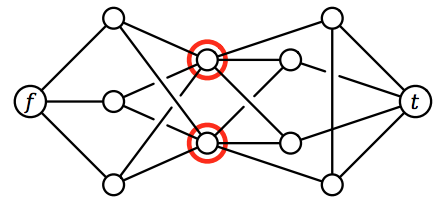
\includegraphics[scale=.75]{images/problem3}
\end{figure}

\solution\\

\begin{algorithm}
	\begin{algorithmic}[1]
		\Function{MinStationClosures}{$G, f, t$}
			\State $N \gets$ a new graph
			\ForAll{$v$ in $G.vertices$}
				\If{$v = f \vee v = t$}
					\State add $v$ to $N$
				\Else
					\State add $v_i$ and $v_o$ to $N$
					\State connect $v_i \rightarrow v_o$ with weight $1$
				\EndIf
			\EndFor
			\ForAll{$v$ in $G.vertices$}
				\ForAll{$w$ in $v.neighbors$}
					\If{$\neg(v = t)$}
						\State connect $v_o \rightarrow w_i$ with weight $\infty$
					\EndIf
					\If{$\neg(v = f)$}
						\State connect $w_o \rightarrow v_i$ with weight $\infty$
					\EndIf
				\EndFor
			\EndFor
			\State \Return the minimum cut of $N$
		\EndFunction
	\end{algorithmic}
\end{algorithm}

The minimum-cut algorithm is here assumed to determine the lowest-weighted edges to cut; an inverse assignment can be used if the min-cut algorithm instead prioritizes the highest-capacity edges.\\

This algorithm is designed to duplicate all vertices in $G$ which are not $s$ or $t$. For all $v \in G$ (again, aside from $s$ or $t$), we construct two vertices, $v_i$ and $v_o$. We then construct edges in a directed graph, such that for all nodes $w$ connected to $v$, there exists a connection from $w_o$ to $v_i$ and a connection from $v_o$ to $w_i$. Without loss of generality, we assume $s$ as a source and $t$ as destination; thus, for all neighbors $n$ of $s$, we construct an edge from $s$ to $n_i$; conversely, for all neighbors $n$ of $t$, we construct an edge from $n_o$ to $t$.\\

Having split each vertex into two, we can construct a connection from $v_i$ to $v_o$, and thus all paths from $s$ to $t$ are preserved. Now, we can perform a standard min-cut algorithm; our edge weightings will ensure that the algorithm only selects our newly-created ``vertex'' edges (those from $v_i$ to $v_o$); cutting this edge has the equivalent effect to removing $v$ from the graph, as now all paths from $s$ to $t$ passing through $v$ are broken.\\

There are two stages to the algorithm to analyze for run-time: graph construction and then the min-cut algorithm.\\

Graph construction is straightforward; we re-create the original graph $G$, doubling vertices and edges as we go; since $V$ is $O(E)$, our total run-time here is simply $O(E)$.\\

For the min-cut algorithm, the fastest algorithm for computing maximum flows is $O(VE)$, as discovered by James Orlin. Since the min-cut is equivalent to the maximum flow, we can use this algorithm to determine the min-cut of our new graph.\\

Thus, the total runtime of our algorithm is $O(VE)$.

\end{homeworkProblem}

\pagebreak

\begin{homeworkProblem}

Suppose we are given an $n \times n$ square grid, some of whose squares are colored black and the rest white. Describe and analyze an algorithm to determine whether tokens can be placed on the grid so that

\begin{enumerate}
\item every token is on a white square;
\item every row of the grid contains exactly one token; and
\item every column of the grid contains exactly one token
\end{enumerate}

\begin{figure}[h]
	\centering
		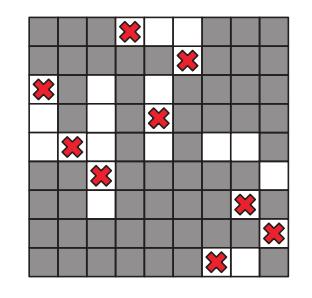
\includegraphics[scale=.75]{images/problem4}
\end{figure}

Your input is a two dimensional array $IsWhite$[1..$n$, 1..$n$] of booleans, indicated which squares are white. Your output is a single boolean. For example, given the grid above as input, your algorithm should return \alg{True}. \\

\solution\\

Solution

\end{homeworkProblem}

\pagebreak

\begin{homeworkProblem}

\emph{Ad-hoc} networks are made up of low-powered wireless devices. In principle, these networks can be used on battlefields, in regions that have recently suffered from natural disasters, and in other hard-to-reach areas. The idea is that a large collection of cheap, simple devices could be distributed through the area of interest (for example, by dropping them from an airplane); the devices would then automatically configure themselves into a functioning wireless network.\\

These devices can communicate only within a limited range. We assume all the devices are identical; there is a distance $D$ such that two devices can communicate if and only if the distance between them is at most $D$.\\

We would like our ad-hoc network to be reliable, but because the devices are cheap and low-powered, they frequently fail. If a device detects that it is likely to fail, it should transmit its information to some other $backup$ device within its communication range. We require each device $x$ to have $k$ potential backup devices, all within distance $D$ of $x$; we call
these $k$ devices the \textbf{\textit{backup set}} of x. Also, we do not want any device to be in the backup set of too many other devices; otherwise, a single failure might affect a large fraction of the network. \\

So suppose we are given the communication radius $D$, parameters $b$ and $k$, and an array $d$[1 .. $n$, 1 .. $n$] of distances, where $d[i, j]$ is the distance between device $i$ and device $j$. Describe an algorithm that either computes a backup set of size $k$ for each of the $n$ devices, such that no device appears in more than $b$ backup sets, or reports (correctly) that
no good collection of backup sets exists. \\

\solution\\

Solution

\end{homeworkProblem}

\end{document}